\documentclass[11pt]{article}
\usepackage[margin=1in]{geometry}\usepackage{amsmath,amssymb,booktabs,graphicx,xcolor}\usepackage[numbers,sort&compress]{natbib}
\usepackage[colorlinks=true,linkcolor=blue!50!black,citecolor=blue!50!black,urlcolor=blue!50!black]{hyperref}\usepackage{url}
\usepackage{caption}\captionsetup{font=small,labelfont=bf}\usepackage{placeins}
\title{Uncertainty Quantification for Tabular Regression:\\ a Benchmark on the Sediment load Dataset}
\author{Prakriti Bisht \and Danesh Selwal}
\date{Regression UQ Analysis v2.0 --- November 2026}
\begin{document}\maketitle
\begin{abstract}We benchmark uncertainty quantification (UQ) methods for tabular regression on the sediment load dataset (1095 training and 365 test samples, 3 features). Ten gradient-boosted, probabilistic and neural regressors are tuned with Optuna and then wrapped by quantile regression, distributional methods (NGBoost, PGBM, IBUG, Treeffuser, CARD), split, cross and bootstrap conformal prediction (MAPIE, PUNCC), weighted and online conformal methods (NexCP, ACI, FACI, SF-OGD, SAOCP, MFCS, COP, Extreme CP), adaptive coverage policies (ACP) and hyperspherical confidence mapping (HCM). At a nominal 90\% level, raw quantile regression reaches a median coverage of only 81.1\%, while conformal methods restore validity; the narrowest method that is valid on most models is NexCP J+aB (median coverage 89.3\%, median width 0.24 target standard deviations). All experiments ran on Kaggle; the executed notebooks and raw outputs are linked from this report.\end{abstract}

\section{Introduction}
A point prediction says nothing about how far the truth may be from it. Uncertainty quantification attaches to each prediction either a predictive distribution or a prediction interval $[\ell(x),u(x)]$ that should contain the true response with a chosen probability $1-\alpha$. Methods differ in their guarantees: quantile regression and parametric distributional models are only asymptotically or approximately calibrated, while conformal prediction gives finite-sample, distribution-free marginal coverage under exchangeability \citep{vovk2005alrw,lei2018distribution,angelopoulos2023gentle}. This report applies one common, fixed pipeline of eight notebooks to the sediment load dataset and compares the methods on coverage, interval width and proper scoring rules. Companion reports with the same structure cover the other eight datasets of the project.

\section{Data}
The training set has 1095 rows and the test set 365 rows. The 3 input features are \texttt{Qt}, \texttt{Qt-1}, \texttt{St-1}; the target is \texttt{St}. On the test set the target has mean 369.0, standard deviation 1,235, median 23.00 and range 0.130--7,400. The train/test split is the one supplied with the data; the test set is used only for the final evaluation (never for tuning or calibration).

\section{Methods}
\subsection{Point predictors and tuning}
Ten regressors are used as base models: random forest \citep{breiman2001rf}, gradient boosting \citep{friedman2001gbm}, histogram gradient boosting \citep{pedregosa2011sklearn}, XGBoost \citep{chen2016xgboost}, LightGBM \citep{ke2017lightgbm}, CatBoost \citep{prokhorenkova2018catboost}, GPBoost \citep{sigrist2022gpboost}, NGBoost \citep{duan2020ngboost}, PGBM \citep{sprangers2021pgbm} and TabNet \citep{arik2021tabnet}. Hyperparameters are tuned with Optuna \citep{akiba2019optuna} by minimising 5-fold cross-validated RMSE on the training set; for each model the best of several pruners (median, Hyperband \citep{li2018hyperband}, Wilcoxon, none) is kept. Random forest is used only in tuning.

\subsection{Quantile regression}
Each boosted model is fitted to the pinball loss $\rho_\tau(r)=r\,(\tau-\mathbb{1}\{r<0\})$ \citep{koenker1978quantile} for $\tau\in\{0.05,\dots,0.95\}$; the 90\% interval is $[\hat q_{0.05}(x),\hat q_{0.95}(x)]$. Separately fitted quantiles can cross \citep{chernozhukov2010rearrangement}; we report the crossing rate.

\subsection{Distributional methods}
NGBoost and PGBM output a Gaussian $\mathcal N(\hat\mu(x),\hat\sigma^2(x))$. IBUG \citep{brophy2022ibug} estimates $\hat\sigma(x)$ from the training targets of the $k$ most affine training points of a boosted ensemble. Treeffuser \citep{beltranvelez2024treeffuser} learns a conditional diffusion with boosted trees and CARD \citep{han2022card} a conditional denoising diffusion model \citep{ho2020ddpm}; samples are summarised by their mean and standard deviation. Every predictive distribution is scored with the continuous ranked probability score \citep{gneiting2007scoring,hersbach2000crps}, which for a Gaussian is
\begin{equation}
\mathrm{CRPS}(\mathcal N(\mu,\sigma^2),y)=\sigma\Big[z\,(2\Phi(z)-1)+2\varphi(z)-\tfrac{1}{\sqrt\pi}\Big],\quad z=\tfrac{y-\mu}{\sigma},
\end{equation}
and the 90\% interval is $\hat\mu\pm1.645\hat\sigma$. PIT histograms and calibration curves \citep{gneiting2007sharpness,kuleshov2018calibrated} are in the notebooks.

\subsection{Conformal prediction}
\emph{Split conformal} \citep{vovk2005alrw,lei2018distribution} holds out a calibration set $\mathcal C$, computes scores $s_i=|y_i-\hat f(x_i)|$ and returns $\hat f(x)\pm\hat q$, with $\hat q$ the $\lceil(1-\alpha)(|\mathcal C|+1)\rceil$-th smallest score; then $P(Y\in\hat C(X))\ge1-\alpha$ for exchangeable data. \emph{CV+} and \emph{jackknife+-after-bootstrap} (J+aB) reuse all data through out-of-fold residuals \citep{barber2021jackknife,kim2020jab}, with guarantee $1-2\alpha$. \emph{CQR} conformalises quantile regression with score $\max\{\hat q_{\alpha/2}(x)-y,\,y-\hat q_{1-\alpha/2}(x)\}$ \citep{romano2019cqr}. We use MAPIE \citep{taquet2022mapie} and PUNCC \citep{mendil2023puncc}.

\emph{NexCP} \citep{barber2023beyond} replaces the empirical quantile by a weighted one, $\hat q=Q_{1-\alpha}\big(\sum_i\tilde w_i\delta_{s_i}+\tilde w_{n+1}\delta_{+\infty}\big)$ with weights decaying in time, and keeps a coverage guarantee degraded by the total-variation drift; it is applied in split, full, CV+ and J+aB form. The \emph{online} methods process the test points sequentially and update the miscoverage level after each observation: ACI \citep{gibbs2021aci} uses
\begin{equation}
\alpha_{t+1}=\alpha_t+\gamma\,(\alpha-\mathrm{err}_t),\qquad \mathrm{err}_t=\mathbb 1\{y_t\notin\hat C_t(x_t)\},
\end{equation}
FACI \citep{gibbs2024faci} aggregates a grid of step sizes $\gamma$, SF-OGD and SAOCP \citep{bhatnagar2023saocp,orabona2018scalefree} run scale-free and strongly adaptive online gradient descent on the quantile directly, MFCS is a split/full online variant, and COP \citep{hu2026cop} uses the predicted distribution to inform the online update. Extreme CP \citep{pasche2025extreme} fits a generalised Pareto tail \citep{pickands1975gpd} to the scores and returns a one-sided upper bound. AlphaNet results are kept in the notebooks only.

\subsection{Adaptive coverage policies and HCM}
ACP \citep{gauthier2026acp} lets a policy choose a per-point level $\tilde\alpha(x)$ and builds the set from conformal e-values \citep{vovk2021evalues,gauthier2025evalues}, so the guarantee holds for the data-dependent level; the realised coverage must be compared with the learned target, not with 90\%. HCM \citep{choi2026hcm} trains a single network whose output direction on a hypersphere encodes the prediction and whose norm encodes confidence; we report its 95\% interval.

\subsection{Evaluation}
With $n=365$ test points the empirical coverage of a correct 90\% method has standard error $\sqrt{0.09/n}=0.016$, so we call an interval \emph{valid} if its coverage is at least $0.9-1.645\sqrt{0.09/n}=0.874$. Among valid methods, narrower is better. Widths are also given relative to the test-target standard deviation so that datasets can be compared. All runs use $\alpha=0.1$ unless stated.

\section{Experimental setup}
All notebooks ran on Kaggle CPU machines with the generalised v2.0 code (every change is listed in \texttt{docs/CHANGELOG\_FIXES.md}). Downstream notebooks load the parameters of the tuning run. Optuna search is not bit-reproducible between runs; the stored tuning run is the one used by every other phase. NB6 was not run for TabNet, PGBM: these jobs exceed Kaggle's 12-hour limit (not enough compute). NexCP Full conformal (a grid search over candidate labels) was switched off for this dataset for the same reason. The executed notebooks are linked in Table~\ref{tab:runs}.

\section{Results}
\begin{table}[t]\centering\small
\caption{Tuned point predictors, sorted by 5-fold cross-validated RMSE on the training set. $r$: Pearson correlation on the test set.}\label{tab:tuning}
\begin{tabular}{llrrr}\toprule Model & Pruner & CV RMSE & Test RMSE & Test $r$\\\midrule
TabNet & NopPruner & 1,925 & 728.5 & 0.962 \\
GradientBoosting & NopPruner & 2,364 & 328.6 & 0.965 \\
RandomForest & WilcoxonPruner & 2,476 & 543.8 & 0.956 \\
GPBoost & WilcoxonPruner & 2,586 & 338.2 & 0.965 \\
LightGBM & HyperbandPruner & 2,596 & 454.0 & 0.963 \\
PGBM & WilcoxonPruner & 2,620 & 440.9 & 0.938 \\
HistGB & MedianPruner & 2,631 & 420.2 & 0.965 \\
NGBoost & WilcoxonPruner & 2,640 & 673.3 & 0.932 \\
XGBoost & WilcoxonPruner & 2,723 & 696.3 & 0.958 \\
CatBoost & NopPruner & 2,762 & 482.7 & 0.925 \\
\bottomrule\end{tabular}\end{table}
\begin{table}[t]\centering\small
\caption{Quantile regression and distributional methods at the 90\% level. For distributional methods the interval is $\hat\mu\pm1.645\hat\sigma$ and the CRPS is the closed-form Gaussian CRPS of $(\hat\mu,\hat\sigma)$; for quantile regression the CRPS is the pinball-loss approximation over the predicted quantiles. Crossing: share of test points whose predicted quantiles are not monotone.}\label{tab:dist}
\begin{tabular}{llrrrr}\toprule Method & Model & Coverage & Width & CRPS & Crossing\\\midrule
QR & TabNet & 89.3\% & 597.2 & 69.97 & 98.6\%\\
QR & CatBoost & 78.6\% & 559.6 & 71.48 & 92.9\%\\
QR & GradientBoosting & 78.1\% & 512.3 & 73.86 & 89.9\%\\
QR & GPBoost & 84.1\% & 767.9 & 75.59 & 68.5\%\\
QR & HistGB & 77.0\% & 523.1 & 79.67 & 99.5\%\\
QR & XGBoost & 81.1\% & 1,176 & 83.76 & 97.3\%\\
QR & LightGBM & 83.8\% & 1,001 & 88.00 & 23.0\%\\
QR & PGBM & 5.8\% & 8.32 & 113.4 & 0.0\%\\
QR & NGBoost & 84.9\% & 277.7 & 128.5 & 0.0\%\\
Native & PGBM & 6.6\% & 8.65 & 113.2 & --\\
Native & NGBoost & 85.8\% & 297.1 & 166.7 & --\\
IBUG & LightGBM & 98.6\% & 1,875 & 178.8 & --\\
IBUG & XGBoost & 98.4\% & 2,450 & 260.4 & --\\
Treeffuser & CatBoost & 99.7\% & 5,623 & 433.3 & --\\
Treeffuser & GradientBoosting & 100.0\% & 5,656 & 441.2 & --\\
Treeffuser & XGBoost & 100.0\% & 6,735 & 553.2 & --\\
Treeffuser & GPBoost & 100.0\% & 22,837 & 1,687 & --\\
Treeffuser & LightGBM & 100.0\% & 50,207 & 3,660 & --\\
CARD & GPBoost & 94.2\% & 561.5 & 64.54 & --\\
CARD & GradientBoosting & 94.2\% & 490.7 & 70.60 & --\\
CARD & HistGB & 94.2\% & 456.7 & 71.78 & --\\
CARD & CatBoost & 95.6\% & 536.6 & 76.39 & --\\
CARD & LightGBM & 94.2\% & 616.3 & 76.54 & --\\
CARD & TabNet & 94.8\% & 631.4 & 77.00 & --\\
CARD & XGBoost & 95.1\% & 538.8 & 78.74 & --\\
CARD & PGBM & 91.8\% & 349.1 & 103.9 & --\\
CARD & NGBoost & 89.9\% & 189.0 & 141.3 & --\\
\bottomrule\end{tabular}\end{table}
\begin{figure}[t]\centering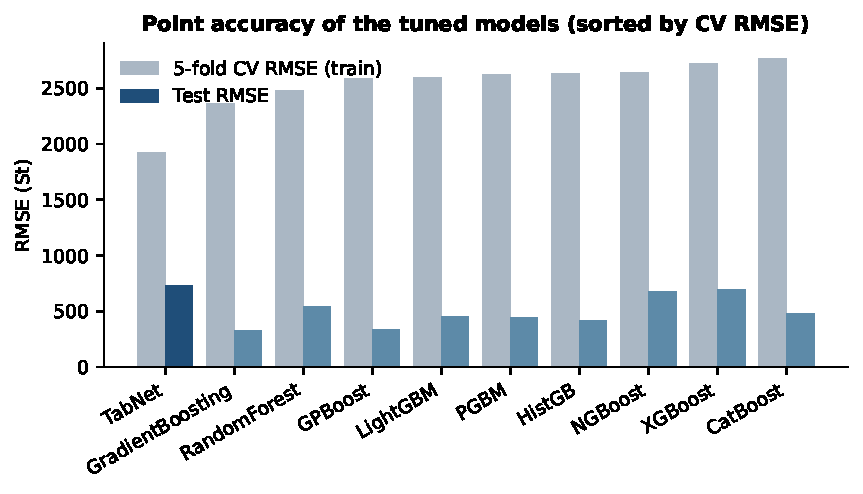
\includegraphics[width=\linewidth]{figures/fig_accuracy.pdf}\caption{Cross-validated and test RMSE of the tuned models. Dark bar: best CV model (TabNet).}\label{fig:acc}\end{figure}
\begin{figure}[t]\centering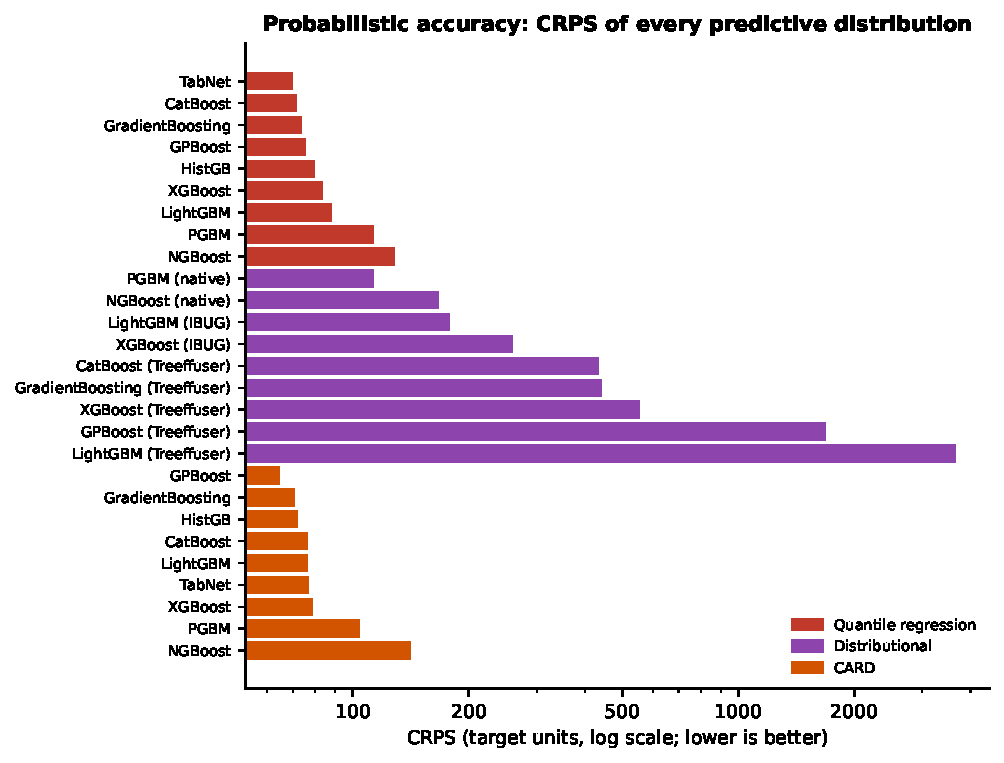
\includegraphics[width=0.9\linewidth]{figures/fig_crps.pdf}\caption{CRPS of every predictive distribution (log scale).}\label{fig:crps}\end{figure}
\paragraph{Point accuracy (Table~\ref{tab:tuning}, Fig.~\ref{fig:acc}).} Point accuracy: TabNet has the lowest 5-fold CV RMSE (1,925); on the test set the lowest RMSE is GradientBoosting (328.6, target std 1,235).
\paragraph{Quantile and distributional methods (Table~\ref{tab:dist}, Fig.~\ref{fig:crps}).} Raw quantile regression undercovers: median 90\%-interval coverage 81.1\% (range 5.8\%--89.3\%); 1 of 9 models reach the target. Quantile crossing occurs on a median 89.9\% of test points. Best probabilistic score: GPBoost (CARD) with CRPS 64.54. NGBoost (native) predictive distributions are over-confident here: the Gaussian 90\% interval covers only 85.8\%. PGBM (native) predictive distributions are over-confident here: the Gaussian 90\% interval covers only 6.6\%. CARD (diffusion) intervals: median coverage 94.2\% at 0.43$\times$ the target std.

\begin{table}[p]\centering\small
\caption{All interval methods at the 90\% target, aggregated over the base models they wrap ($n$). Width: median over models of the mean test-interval width; rel.: divided by the standard deviation of the test target. $^\dagger$: some intervals reach the edge of the label grid, so the reported width is a lower bound; the method is not ranked. Valid: share of models whose coverage is at least $0.9-1.645\sqrt{0.09/n_{\text{test}}}=0.874$.}\label{tab:league}
\resizebox{\textwidth}{!}{\begin{tabular}{llrrcrrr}\toprule Family & Method & $n$ & Coverage (median) & Range & Width & Rel. & Valid\\\midrule
Quantile regression & Quantile regression (raw) & 9 & 81.1\% & 5.8\%--89.3\% & 559.6 & 0.45 & 11\% \\
Distributional & PGBM (native) & 1 & 6.6\% & 6.6\%--6.6\% & 8.65 & 0.01 & 0\% \\
Distributional & NGBoost (native) & 1 & 85.8\% & 85.8\%--85.8\% & 297.1 & 0.24 & 0\% \\
Distributional & IBUG & 2 & 98.5\% & 98.4\%--98.6\% & 2,163 & 1.75 & 100\% \\
Distributional & Treeffuser & 5 & 100.0\% & 99.7\%--100.0\% & 6,735 & 5.45 & 100\% \\
CARD & CARD & 9 & 94.2\% & 89.9\%--95.6\% & 536.6 & 0.43 & 100\% \\
Conformal (MAPIE/PUNCC) & CQR (PUNCC) & 9 & 91.5\% & 75.6\%--96.2\% & 748.1 & 0.61 & 78\% \\
Conformal (MAPIE/PUNCC) & J+aB (MAPIE) & 9 & 94.5\% & 93.2\%--96.7\% & 988.0 & 0.80 & 100\% \\
Conformal (MAPIE/PUNCC) & Split CP (PUNCC) & 9 & 93.4\% & 81.4\%--93.7\% & 1,127 & 0.91 & 89\% \\
Conformal (MAPIE/PUNCC) & CV+ (PUNCC) & 9 & 96.7\% & 94.5\%--99.7\% & 1,242 & 1.01 & 100\% \\
Conformal (MAPIE/PUNCC) & Split CP (MAPIE) & 9 & 95.6\% & 84.4\%--97.0\% & 1,364 & 1.10 & 89\% \\
Conformal (MAPIE/PUNCC) & CV+ (MAPIE) & 9 & 97.8\% & 94.0\%--99.7\% & 2,046 & 1.66 & 100\% \\
Weighted conformal (NexCP) & NexCP Split & 7 & 88.8\% & 86.6\%--90.4\% & 270.6 & 0.22 & 71\% \\
Weighted conformal (NexCP) & NexCP J+aB & 7 & 89.3\% & 87.9\%--91.0\% & 298.8 & 0.24 & 100\% \\
Weighted conformal (NexCP) & NexCP CV+ & 7 & 92.1\% & 91.2\%--94.8\% & 467.1 & 0.38 & 100\% \\
Online conformal & ACI & 7 & 92.3\% & 92.1\%--93.4\% & 551.6 & 0.45 & 100\% \\
Online conformal & FACI & 7 & 92.3\% & 91.0\%--92.6\% & 871.5 & 0.71 & 100\% \\
Online conformal & Online J+aB & 7 & 94.0\% & 93.7\%--95.3\% & 885.5 & 0.72 & 100\% \\
Online conformal & MFCS Full & 7 & 93.7\% & 92.9\%--94.2\% & 903.3 & 0.73 & 100\% \\
Online conformal & MFCS Split & 7 & 94.2\% & 92.9\%--95.6\% & 1,104 & 0.89 & 100\% \\
Online conformal & Online Split & 7 & 94.2\% & 92.9\%--95.6\% & 1,104 & 0.89 & 100\% \\
Online conformal & Online CV+ & 7 & 95.9\% & 94.8\%--98.1\% & 1,153 & 0.93 & 100\% \\
Online conformal & SF-OGD & 7 & 90.1\% & 89.9\%--90.1\% & 5,064 & 4.10 & 100\% \\
Online conformal & SAOCP & 7 & 99.5\% & 99.5\%--100.0\% & 10,539 & 8.53 & 100\% \\
COP & COP & 7 & 95.9\% & 94.8\%--96.7\% & 1,029 & 0.83 & 100\% \\
\bottomrule\end{tabular}}\end{table}
\begin{figure}[t]\centering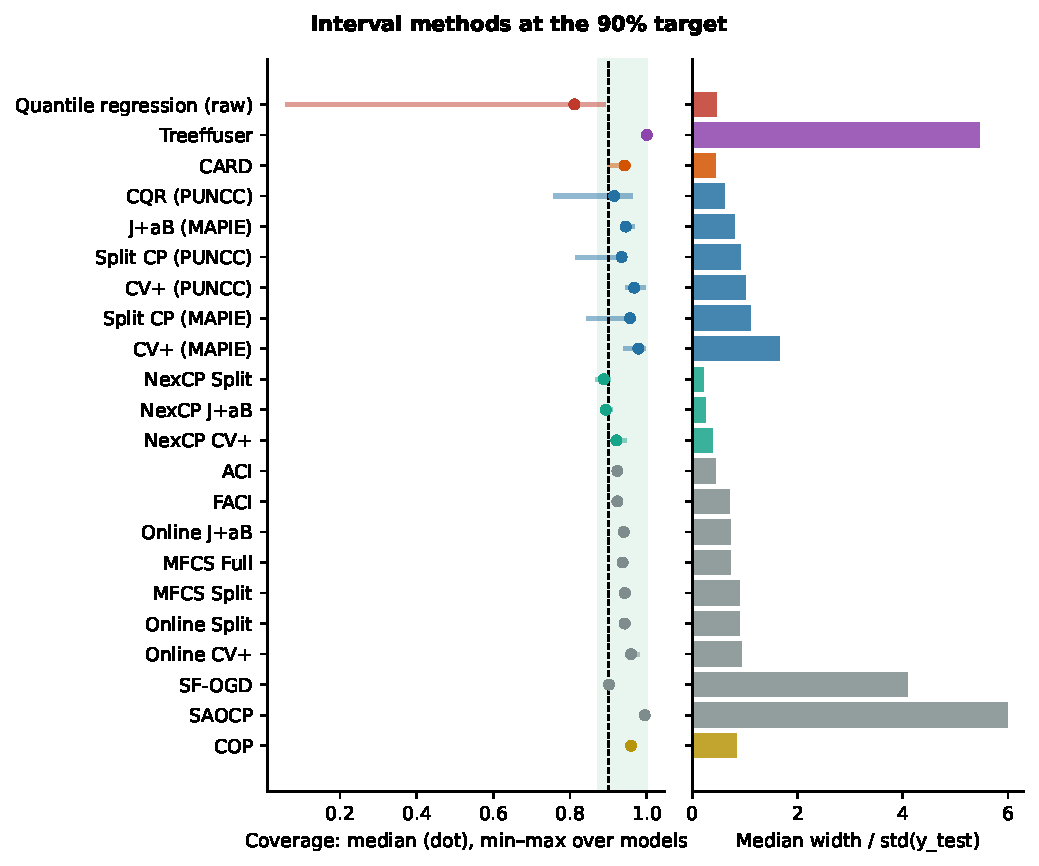
\includegraphics[width=0.95\linewidth]{figures/fig_method_league.pdf}\caption{Coverage (left; band: valid region) and relative width (right) of every interval method, aggregated over base models.}\label{fig:league}\end{figure}
\begin{figure}[t]\centering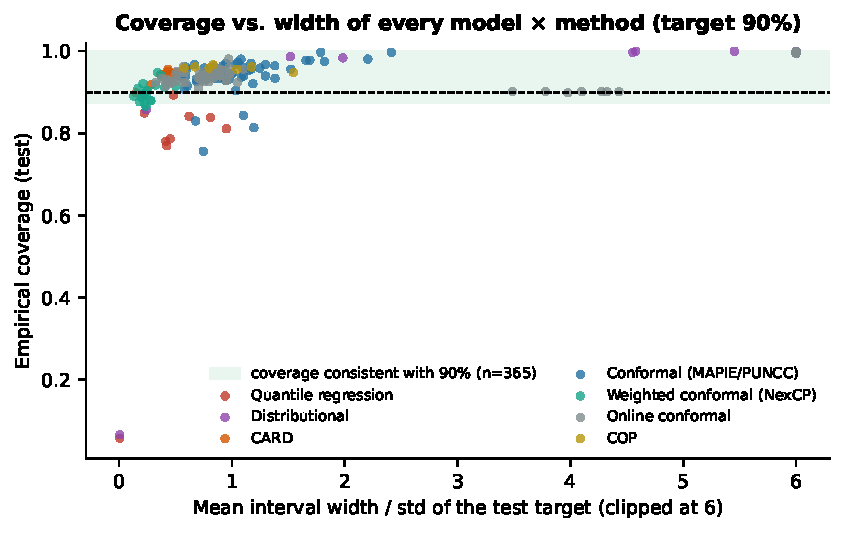
\includegraphics[width=0.9\linewidth]{figures/fig_coverage_width.pdf}\caption{Coverage against relative width for every base model $\times$ method pair. Good methods sit in the shaded band at the far left.}\label{fig:cw}\end{figure}
\begin{figure}[t]\centering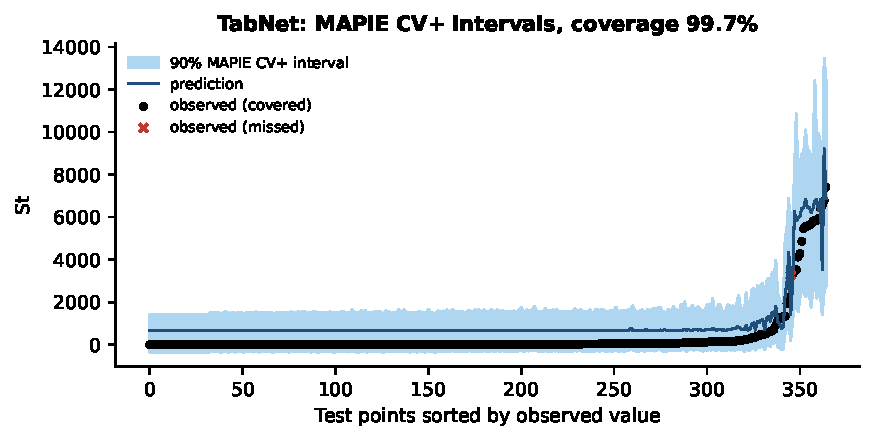
\includegraphics[width=0.9\linewidth]{figures/fig_intervals.pdf}\caption{MAPIE CV+ 90\% intervals of TabNet on the test set, sorted by observed value; red crosses are misses.}\label{fig:int}\end{figure}
\paragraph{Interval methods (Table~\ref{tab:league}, Figs.~\ref{fig:league}--\ref{fig:int}).} Recommended interval method: NexCP J+aB -- the narrowest method that reaches the 90\% target (within sampling tolerance, n=365) on $\geq$75\% of models: median coverage 89.3\%, median width 298.8 (0.24$\times$ target std). Narrowest single valid interval (coverage within tolerance of 90\%): NexCP Split on GradientBoosting, coverage 89.0\%, mean width 162.8. Among valid intervals, median width / target std by family: Weighted conformal (NexCP) 0.24; CARD 0.43; Quantile regression 0.48; Online conformal 0.81; COP 0.83; Conformal (MAPIE/PUNCC) 0.99; Distributional 4.58.

\begin{table}[t]\centering\small
\caption{Extreme conformal prediction: one-sided upper bound $\hat y+q$ (no lower bound). Coverage is $P(y\le \hat y+q)$; the last column is $q$.}\label{tab:extreme}
\begin{tabular}{lrr}\toprule Model & Coverage & $q$\\\midrule
CatBoost & 97.5\% & 425.0\\
GPBoost & 97.8\% & 222.6\\
GradientBoosting & 97.3\% & 233.7\\
HistGB & 95.1\% & 404.3\\
LightGBM & 98.6\% & 563.2\\
NGBoost & 97.5\% & 331.2\\
XGBoost & 97.3\% & 279.8\\
\bottomrule\end{tabular}\end{table}
\begin{table}[t]\centering\small
\caption{Adaptive coverage policies: mean learned target coverage $1-\tilde\alpha$, realised coverage and width of the e-value prediction sets.}\label{tab:acp}
\begin{tabular}{lrrrrr}\toprule Model & Target & Coverage & Width & RMSE & $\lambda$\\\midrule
CatBoost & 0.1\% & 92.1\% & 704.8 & 486.4 & 50.00\\
GPBoost & 0.1\% & 92.6\% & 563.8 & 368.6 & 50.00\\
GradientBoosting & 0.1\% & 93.4\% & 521.3 & 377.4 & 50.00\\
HistGB & 0.1\% & 90.4\% & 679.6 & 915.0 & 50.00\\
LightGBM & 0.1\% & 93.2\% & 609.9 & 361.2 & 50.00\\
NGBoost & 0.1\% & 91.8\% & 532.3 & 493.0 & 50.00\\
PGBM & 0.1\% & 93.7\% & 742.1 & 390.1 & 50.00\\
TabNet & 0.1\% & 93.7\% & 905.2 & 462.4 & 50.00\\
XGBoost & 0.1\% & 91.5\% & 792.5 & 609.3 & 50.00\\
\bottomrule\end{tabular}\end{table}
\begin{table}[t]\centering\small
\caption{Hyperspherical confidence mapping (one network).}\label{tab:hcm}
\begin{tabular}{lr}\toprule Metric & Value\\\midrule
Coverage of 95\% interval & 100.0\%\\
Mean 95\% width & 3,819\\
Coverage at $1\sigma$ & 44.4\%\\
Coverage at $2\sigma$ & 100.0\%\\
Coverage at $3\sigma$ & 100.0\%\\
RMSE & 911.4\\
MAE & 755.9\\
CRPS & 489.0\\
NLL & 8.06\\
Spearman (|error|, $\sigma$) & -0.573\\
Regression ECE & 279.8\\
\bottomrule\end{tabular}\end{table}
\paragraph{Extreme CP, ACP and HCM.} ACP policy saturated at the boundary $\tilde\alpha$ = 0.999 for 9 of 9 models (CatBoost, GPBoost, GradientBoosting, HistGB, LightGBM, NGBoost, PGBM, TabNet, XGBoost): the sets have constant width and the learned level carries no information; realised coverage 90.4\%--93.7\%. HCM (single network, 95\% interval): coverage 100.0\%, RMSE 911.4, error--uncertainty Spearman correlation -0.57. Extreme CP returns only an upper bound (Table~\ref{tab:extreme}), so it is not ranked with two-sided intervals.

\FloatBarrier
\section{Conclusions}
\begin{itemize}\setlength\itemsep{2pt}
\item Point accuracy: TabNet has the lowest 5-fold CV RMSE (1,925); on the test set the lowest RMSE is GradientBoosting (328.6, target std 1,235).
\item Raw quantile regression undercovers: median 90\%-interval coverage 81.1\% (range 5.8\%--89.3\%); 1 of 9 models reach the target. Quantile crossing occurs on a median 89.9\% of test points.
\item Best probabilistic score: GPBoost (CARD) with CRPS 64.54.
\item NGBoost (native) predictive distributions are over-confident here: the Gaussian 90\% interval covers only 85.8\%.
\item PGBM (native) predictive distributions are over-confident here: the Gaussian 90\% interval covers only 6.6\%.
\item CARD (diffusion) intervals: median coverage 94.2\% at 0.43$\times$ the target std.
\item Recommended interval method: NexCP J+aB -- the narrowest method that reaches the 90\% target (within sampling tolerance, n=365) on $\geq$75\% of models: median coverage 89.3\%, median width 298.8 (0.24$\times$ target std).
\item Narrowest single valid interval (coverage within tolerance of 90\%): NexCP Split on GradientBoosting, coverage 89.0\%, mean width 162.8.
\item Among valid intervals, median width / target std by family: Weighted conformal (NexCP) 0.24; CARD 0.43; Quantile regression 0.48; Online conformal 0.81; COP 0.83; Conformal (MAPIE/PUNCC) 0.99; Distributional 4.58.
\item ACP policy saturated at the boundary $\tilde\alpha$ = 0.999 for 9 of 9 models (CatBoost, GPBoost, GradientBoosting, HistGB, LightGBM, NGBoost, PGBM, TabNet, XGBoost): the sets have constant width and the learned level carries no information; realised coverage 90.4\%--93.7\%.
\item HCM (single network, 95\% interval): coverage 100.0\%, RMSE 911.4, error--uncertainty Spearman correlation -0.57.
\item Not run (out of compute, Kaggle 12-hour limit): NB6 for TabNet, PGBM.
\item NexCP Full conformal was not run on this dataset (out of compute).
\end{itemize}
\paragraph{Limitations.} One fixed train/test split is used, so all coverages carry the sampling error stated above; widths are compared on the same split. The online methods treat the test set as a sequence in its stored order. Optuna tuning is not bit-reproducible. CARD, HCM and TabNet are neural and sensitive to their seeds.

\paragraph{Reproducibility.} Code: \url{https://github.com/DaneshSelwal/Regression_Uncertainty_Quantification_Analysis} (branch \texttt{version2.0}), folder \texttt{examples/sediment\_load\_uncertainty\_analysis}. Every executed notebook is stored next to its Excel outputs and is listed below.
\begin{table}[h]\centering\scriptsize\caption{Kaggle runs whose outputs are reported here.}\label{tab:runs}
\begin{tabular}{lll}\toprule Notebook & Run & Kaggle URL\\\midrule
NB1 & \texttt{REG22\_11\_2026\_17\_58} & \url{https://www.kaggle.com/code/daneshselwal/reg22-11-2026-17-58}\\
NB2 & \texttt{REG23\_11\_2026\_01\_24} & \url{https://www.kaggle.com/code/daneshjangra/reg23-11-2026-01-24}\\
NB3 & \texttt{REG23\_11\_2026\_01\_25} & \url{https://www.kaggle.com/code/daneshjangra/reg23-11-2026-01-25}\\
NB4 & \texttt{REG23\_11\_2026\_01\_34} & \url{https://www.kaggle.com/code/daneshjangra/reg23-11-2026-01-34}\\
NB5 & \texttt{REG23\_11\_2026\_01\_37} & \url{https://www.kaggle.com/code/daneshjangra/reg23-11-2026-01-37}\\
NB6 & \texttt{REG23\_11\_2026\_13\_40} & \url{https://www.kaggle.com/code/daneshjangra/reg23-11-2026-13-40}\\
NB6 & \texttt{REG23\_11\_2026\_14\_42} & \url{https://www.kaggle.com/code/daneshselwal/reg23-11-2026-14-42}\\
NB6 & \texttt{REG23\_11\_2026\_14\_49} & \url{https://www.kaggle.com/code/daneshselwal/reg23-11-2026-14-49}\\
NB6 & \texttt{REG23\_11\_2026\_14\_54} & \url{https://www.kaggle.com/code/daneshselwal/reg23-11-2026-14-54}\\
NB6 & \texttt{REG23\_11\_2026\_15\_01} & \url{https://www.kaggle.com/code/daneshselwal/reg23-11-2026-15-01}\\
NB6 & \texttt{REG23\_11\_2026\_15\_04} & \url{https://www.kaggle.com/code/daneshselwal/reg23-11-2026-15-04}\\
NB6 & \texttt{REG23\_11\_2026\_15\_09} & \url{https://www.kaggle.com/code/daneshselwal/reg23-11-2026-15-09}\\
NB7 & \texttt{REG23\_11\_2026\_01\_38} & \url{https://www.kaggle.com/code/daneshjangra/reg23-11-2026-01-38}\\
NB8 & \texttt{REG23\_11\_2026\_01\_45} & \url{https://www.kaggle.com/code/daneshjangra/reg23-11-2026-01-45}\\
\bottomrule\end{tabular}\end{table}

\paragraph{Acknowledgements.} This work was carried out under the guidance of Dr.\ Mahesh Pal.

\FloatBarrier
\bibliographystyle{plainnat}\bibliography{references}
\end{document}
